\section{Power BI 简介}

\subsection{什么是Power BI}

Power BI 是一个微软开发的强大的自助商业智能分析工具。名字中的BI,全称是Business intelligence,即为商业智能。它可以非常方便地用于动态交互式的数据可视化分析与数据展示。如\figref{fig:powerbi}中所示为Power BI平台的操作界面。

\begin{figure}[htbp]
    \centering
    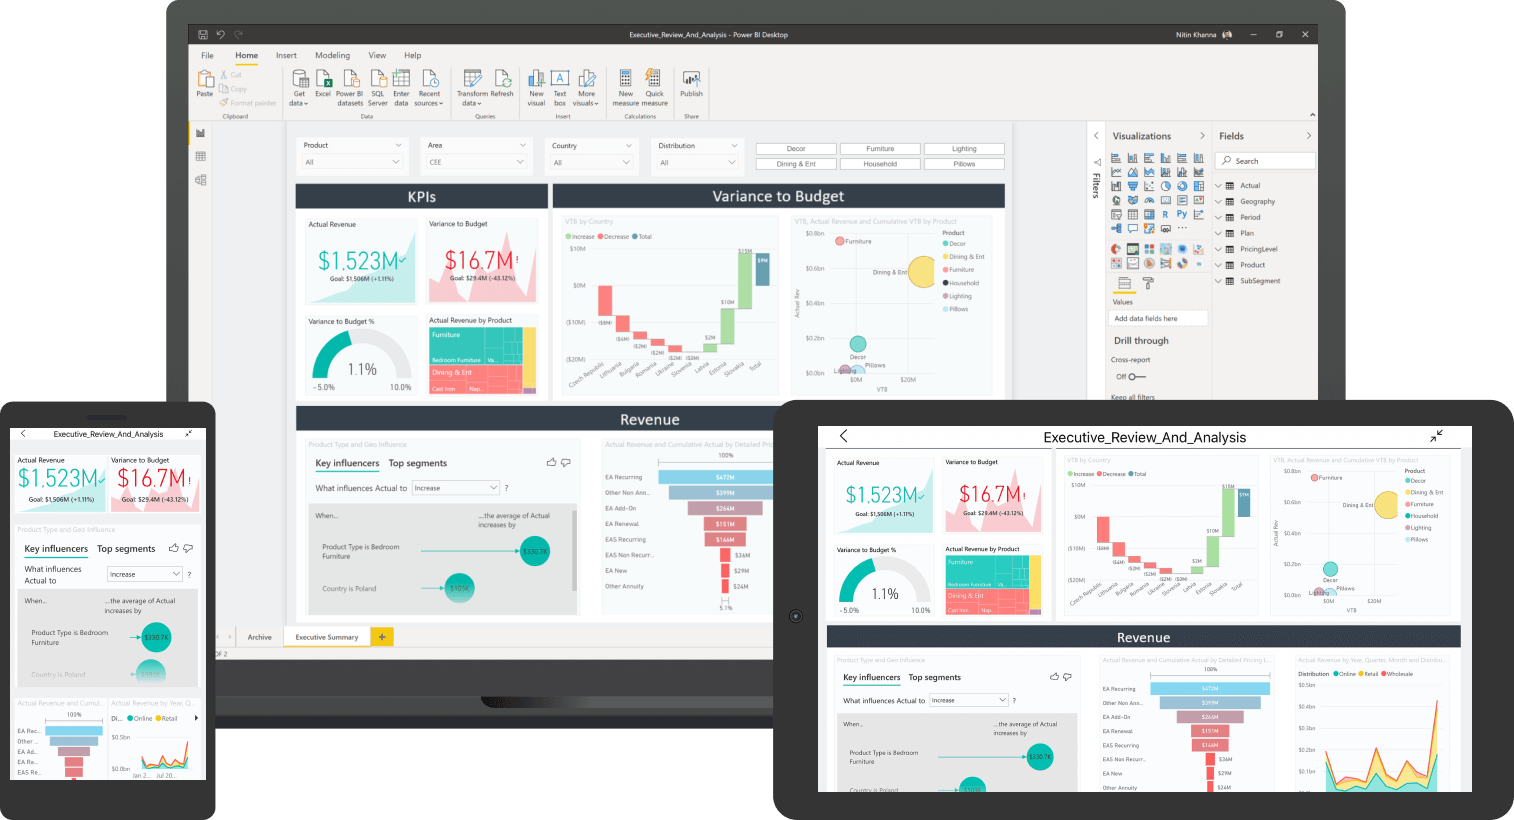
\includegraphics[width=0.9\textwidth]{figure/PowerBI/powerbi.png}
    \caption{\textbf{Power BI 界面}}
    \label{fig:powerbi}
\end{figure}

\subsection{为什么使用 Power BI}

在如今数据分析技能越发重要的时代,许多非数据分析专业人士面对海量的数据,对数据有想法,想发掘出其中的价值来,但可能会因为没有经过专业的训练、没有时间和精力去学习相对复杂的编程,而不知道要怎么样去实践操作数据,心有余而力不足。Power BI便能够为这些用户,也包括了专业的数据分析人士提供了一个自助智能,方便易用且非常强大的数据分析平台。

无需依赖专业技术人员,面对海量的大数据,我们也能够借助Power BI 快速轻松处理和实时全面地发现数据中蕴含的信息,可视化交互展示数据,并分享报表,功能强大。且几乎无门槛的自助使用让数据分析变得简单。Power BI还在效率、性能和对数据量的驾驭上都做到了出色。其主要特点有:

\begin{enumerate}
    \item \textbf{拥有令人赞叹的数据体验:}能够轻松地连接到各种数据源、对数据进行建模和可视化,创建个性化的精美报表。
    \item \textbf{上手快,成本低:}Power BI操作方式和我们熟悉的微软Office的界面很类似,用户能够快速地上手。且对于最核心的Power BI Desktop 应用完全免费,个人可以免费学习和实用,在企业中也能低成本地应用到Power BI的强大功能。
    \item \textbf{与微软的其他产品协作工作:}可以跨常用的 Microsoft Office 应用程序(如 Microsoft Teams 和 Excel 等)轻松地协作处理同一份数据和报表,并能够方便地与他人分享报表和对数据的见解,帮助团队快速作出数据驱动的决策。
    \item \textbf{种类众多的数据连接器:}随着超过 120 个免费连接器库不断扩大,每个人都知道如何实现数据驱动的决策制定。直接连接到数百个本地和云数据源,例如 Dynamics 365、Azure SQL 数据库、MySQL、Excel 和 SharePoint等。
    \item \textbf{AI人工智能辅助:}Power BI面向非数据科学家准备数据,构建机器学习模型,可从结构化和非结构化数据(包括文本和图像)中快速找到用户想要的数据分析结果。
\end{enumerate}

Power BI 在同类软件中也保持着非常大的优势,从国际知名的第三方评估机构Gartner发布的排名情况可了解到微软的Power BI一直以来都处于竞品中的领导者地位,是同类最好的一款BI产品。如\figref{fig:gartner_bi_rank}所示为Gartner在2021年最新发布的BI平台魔力象限图,在分析和商业智能平台领域 Gartner已连续第十四年将 Microsoft 评为领导者。

\begin{figure}[htbp]
    \centering
    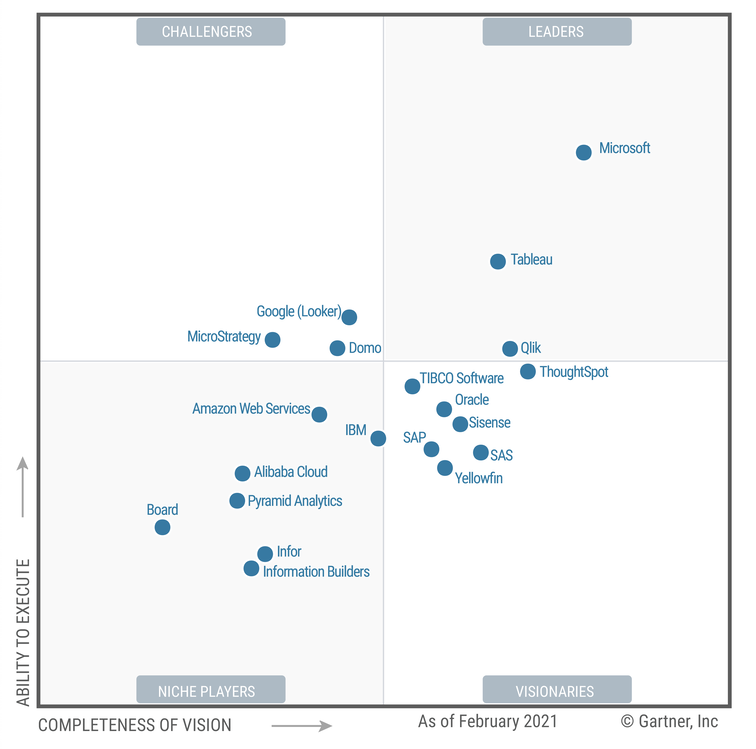
\includegraphics[width=0.6\textwidth]{figure/PowerBI/gartner_bi_rank.png}
    \caption{\textbf{Gartner 2021年 BI 平台魔力象限}}
    \label{fig:gartner_bi_rank}
\end{figure}
